% Define the basic elements of the document
\documentclass[10pt,a4paper]{moderncv}
\moderncvtheme[blue]{classic}

% Change the following variables to set the document overall display
\newcommand{\TopMargin}{0.8cm}
\newcommand{\SideMargin}{0.8cm}
\newcommand{\ItemsSpacing}{0.3cm}
\newcommand{\ItemsMinSpacing}{0.1cm}

% Select the CV language : Native or english (default)
\newif \ifnativelang
%\nativelangtrue % Uncomment to switch to French

% Needed inclusions
\usetikzlibrary{shapes.geometric,calc}
\usepackage[absolute,overlay]{textpos}
\usepackage[utf8]{inputenc}
\usepackage{pdfpages}
\usepackage{tikz}

% Colors used in the template, for coherence
\definecolor{myblack}{rgb}{0,0,0}% black
\definecolor{mylightblue}{rgb}{0.22,0.45,0.70}% light blue
\definecolor{mydarkgrey}{rgb}{0.45,0.45,0.45}% dark grey

\usepackage[scale=0.85, top=\TopMargin, bottom=\TopMargin, right=\SideMargin, left=\SideMargin]{geometry}
\setlength{\hintscolumnwidth}{2.8cm}

% Used for the start system (for skills)
\newcommand\score[2]{
\pgfmathsetmacro\pgfxa{#1+1}
\tikzstyle{scorestars}=[star, star points=5, star point ratio=2.25, draw,inner sep=0.15em,anchor=outer point 3]
\begin{tikzpicture}[baseline]
  \foreach \i in {1,...,#2} {
    \pgfmathparse{(\i<=#1?"color1":"white")}
    \edef\starcolor{\pgfmathresult}
    \draw (\i*1em,0) node[name=star\i,scorestars,fill=\starcolor]  {};
   }
   \pgfmathparse{(#1>int(#1)?int(#1+1):0}
   \let\partstar=\pgfmathresult
   \ifnum\partstar>0
     \pgfmathsetmacro\starpart{#1-(int(#1))}
     \path [clip] ($(star\partstar.outer point 3)!(star\partstar.outer point 2)!(star\partstar.outer point 4)$) rectangle 
    ($(star\partstar.outer point 2 |- star\partstar.outer point 1)!\starpart!(star\partstar.outer point 1 -| star\partstar.outer point 5)$);
     \fill (\partstar*1em,0) node[scorestars,fill=color1]  {};
   \fi

,\end{tikzpicture}
}


% This file contains user's general informations. Modify if necessary
\firstname{Julien}
\familyname{Beaudaux}

\title{ }
%\title{\Large{Research \& Development engineer}}

\mobile{(+33) 06.75.98.14.24}
\email{julienbeaudaux@gmail.com}
\homepage{blueprint-project.info}
\extrainfo{\githubsocialsymbol~\linkedinsocialsymbol~JBeaudaux} %Linkedin and Github

%\extrainfo{Born on March 11th 1986, Married}
%\address{47A Route du G\'en\'eral de Gaulle}{67300 Schiltigheim, FRANCE}

\photo[40pt]{img/profilLight.jpg}



% Optional CV parts to include
\newif \ifreferences
\referencestrue % Uncomment to integrate references

\newif \ifhobbies
%\hobbiestrue % Uncomment to integrate references




%Start CV generation here
\begin{document}
\maketitle

%\begin{minipage}[t]{0.45\textwidth} 

% Header and Skills section. Go to file to modify details
\vspace{-1.3cm}

% Defines the text to use
\ifnativelang
\newcommand{\CVheader}{6 ann\'ees d'exp\'erience en syst\`emes embarqu\'es critiques et r\'eseaux.}% pour applications m\'edicales.\\
%Expérience en conduite d’équipe et normes médicales.}
\else
\newcommand{\CVheader}{6+ years of experience in Real-Time systems, embedded linux and networking.\\
Experience in project steering and team management.}
\fi

%\begin{center}
%\textcolor{color1}{\Large{\CVheader}}
%\end{center}

\section{\ifnativelang Comp\'etences cl\'e\else Key skills\fi}

\ifaddmngt
\subsection{\ifnativelang Comp\'etences techniques\else Technical skills\fi}
\fi

% \cvcomputer{
% \textbf{\ifnativelang Syst\`emes embarqu\'es\else Embedded systems \fi}}{
% \begin{itemize}
% \item \ifnativelang OSs temps-r\'eel \else Real-time OSs \fi : Keil CMSIS, Contiki %ThreadX
% \item \ifnativelang Linux embarqu\'e : U-boot, Busybox\else Embedded Linux : U-boot, Busybox \fi
% \item \ifnativelang Bus de communication \& drivers \else Communication busses and drivers\fi
% \item \ifnativelang D\'eveloppement bas-niveau \else Low-level development\fi
% \item \ifnativelang Tests unitaires, analyse statique \else Unit testing, static analysis \fi (Parasoft)
\cvcomputer{
\textbf{\ifnativelang D\'eveloppement informatique \else Embedded systems \fi}}{
\begin{itemize}
\item Linux, OSX \& syst\`emes temps-r\'eel
\item Connaissances en d\'ev. mobile \& IHM
% \item Connaissances en parall\'elisme
\item Analyse statistique, tests de performance
\end{itemize}
}
{\ifnativelang\textbf{Langages}\else \textbf{Languages}\fi}{
\score{5}{5} MISRA C \\%/ C++\\
\score{4}{5} Python, bash\\
%\score{4}{5} Linux and scripting\\
\score{3}{5} C++ \& Java \\
\score{2}{5} Angular, HTML5, CSS
}

\vspace{\ItemsSpacing}

\cvcomputer{\textbf{\small{\ifnativelang R\'eseaux\else Networking\fi}}}{
\begin{itemize}
\item \ifnativelang Protocoles standards \else Standard protocols \fi : TCP/IP, GSM
\item \ifnativelang Internet des objets \else Internet of things \fi : Sigfox/LoRa, Zigbee
\end{itemize}
}{\textbf{\small{\ifnativelang Contr\^ole qualit\'e\else Quality control\fi}}}{
\begin{itemize}
\item \ifnativelang Int\'egration continue, analyse statique \else Continuous integration, static analysis \fi
\item \ifnativelang Tests unitaires et de performance \else Unit and performance testing\fi
%\item \ifnativelang Normes médicales \else Documentation and medical norms \fi : ISO 62304 \& 62366, CE \& FDA
\end{itemize}}
% }{\textbf{\small{\ifnativelang Recherche \& innovation\else Research \& innovation\fi}}}{
% \begin{itemize}
% \item \ifnativelang 10+ papiers scientifiques (1 best-paper) \else 10+ research articles (1 best-paper award) \fi
% \item \ifnativelang Implication dans l'Open-Source \else Involved in Open-Source projects \fi
% \end{itemize}}

% }{\textbf{\small{\ifnativelang Contr\^ole qualit\'e\else Quality control\fi}}}{
% \begin{itemize}
% \item \ifnativelang Int\'egration continue, analyse statique \else Continuous integration, static analysis \fi
% \item \ifnativelang Tests unitaires et de performance \else Unit and performance testing\fi
% %\item \ifnativelang Normes médicales \else Documentation and medical norms \fi : ISO 62304 \& 62366, CE \& FDA
% \end{itemize}}

\ifaddmngt

\vspace{\ItemsMinSpacing}

\subsection{\ifnativelang Comp\'etences fonctionnelles\else Functional skills\fi}

\cvcomputer{\textbf{\small{\ifnativelang Gestion de projet\else Project steering\fi}}}{
\begin{itemize}
\item \ifnativelang Connaissances en gestion de projet \else Knowledge in project management\fi
\item \ifnativelang Expérience en conduite d'équipes \else Experience in team leadership\fi
\end{itemize}
}{\textbf{\small{\ifnativelang Documentation et normes \else Project steering\fi}}}{
\begin{itemize}
\item \ifnativelang Rédaction des documents applicables \else Applicable documents writing \fi
\item \ifnativelang Normes médicales \else Medical norms \fi : ISO 62304 \& 62366 CE \& FDA
%\item CE Mark (ISO 62304) \& FDA clearance %(21CFR11/820)
%Rédaction de référentiels d'exigences
%Chiffrage projet et participation à la rédaction des propositions commerciales, forte implication en avant-vente
\end{itemize}}

%\cvcomputer{\textbf{\small{\ifnativelang Recherche \& innovation\else Research \& innovation\fi}}}{
%\begin{itemize}
%\item \ifnativelang 10+ papiers scientifiques (1 best-paper) \else 10+ research articles (1 best-paper award) \fi
%\item \ifnativelang Implication dans l'Open-Source \else Involved in Open-Source projects \fi
%\end{itemize}

\fi


\vspace{\ItemsSpacing}

\ifnativelang
\cventry{\textbf{\small{Langues}}}
{Fran\c cais - \textmd{Langue maternelle,} Anglais - \textmd{Courant,} Japonais, Ukrainien - \textmd{Interm\'ediaire}}{}{}{}{}
\else
\cventry{\textbf{\small{Languages}}}
{French - \textmd{Mother tongue,} English - \textmd{Fluent,} Japanese, Ukrainian - \textmd{Intermediate,}  German - \textmd{Beginner}}{}{}{}{}
\fi

%\cventry{\textbf{\small{\ifnativelang Langues\else Languages\fi}}}{\textbf{Fran\c cais} - Langue maternelle, \textbf{Anglais} - Bilingue, \textbf{Japonais} - Avanc\'e, \textbf{Ukrainien} - Interm\'ediaire}{}{}



%\subsection{\ifnativelang Langues\else Languages\fi}
%\ifnativelang
%\hspace{3.1cm}\textbf{Fran\c cais} - Langue maternelle, \textbf{Anglais} - Bilingue, \textbf{Japonais} - Avanc\'e, \textbf{Ukrainien} - Interm\'ediaire
%\else
%\hspace{3.1cm}\textbf{French} - Mother tongue, \textbf{English} - Fluent, \textbf{Japanese} - Advanced, \textbf{Ukrainian} - Intermediate
%\fi







\vspace{\ItemsSpacing}

% Experience section. Go to file to modify details
\section{\ifnativelang Exp\'eriences significatives\else Relevant experiences\fi}

\cventry{11/2014 - Pr\'esent
\raisebox{-6mm}{\href{http://www.schiller.ch/}{
\includegraphics[width=2cm]{img/schiller.png}}}
}{\ifnativelang Ing\'enieur R\&D, Charg\'e de projets logiciels -  Schiller M\'edical\else Lead R\&D engineer - Schiller M\'edical\fi}
{}{}{Wissembourg, France}{
\ifnativelang
	\textcolor{color1}{\textbf{Missions :}}
	\begin{itemize}
		\item \textbf{Participation \`a la mise en \oe uvre et au suivi de projets}
		\begin{itemize}
			\item Conduite d’une équipe de 5 ingénieurs informatique
			\item Chargé du déploiement en production et des qualification hardware et software
			\item Documentation de la partie informatique de projet et contrôle du respect des normes applicables
		\end{itemize}
		\item \textbf{Développement embarqué d'appareils de médecine d’urgence}
		\begin{itemize}
			\item D\'eveloppement MISRA C et C++ sur cibles STM32 et IMX28
			\item D\'eveloppement de modules communicants Lora/Sigfox \& GSM et applications mobiles avec Ionic
			\item Mise en place d'outils d'intégration continue et des processus d'assurance qualit\'e
		\end{itemize}
	\end{itemize}
	\textcolor{color1}{\textbf{Produits :}}
	\begin{itemize}
		\item \textbf{FRED PA-1} : Défibrillateur grand-public connecté \textcolor{color1}{\href{http://www.schiller.ch/fr/fr/product/fred-pa-1}{\ExternalLink}}
		\item \textbf{Open-Heart} : Coach d'activit\'e physique pour r\'ehabilitation cardiaque \textcolor{color1}{\href{http://www.schiller.ch/fr/fr/schiller-\%C3\%A0-la-fine-pointe-de-la-sant\%C3\%A9-connect\%C3\%A9e}{\ExternalLink}}
	\end{itemize}
\else
	\textcolor{color1}{\textbf{Missions :}}
	\begin{itemize}
		\item \textbf{Participation to projects implementation and follow-up}
		\begin{itemize}
			\item Management of a 5-engineers software team
			\item Responsible for production rollout and hardware and software qualification
			\item Documentation of the project software part and control of the applicable norms
		\end{itemize}
		\item \textbf{Embedded software development on emergency medicine devices}
		\begin{itemize}
			\item MISRA C and C++ development on STM32 et IMX28 targets
			\item Development of communication components with Lora/Sigfox \& GSM and mobile applications with Ionic
			\item Implementation of continuous integration tools and quality assurance processes
		\end{itemize}
	\end{itemize}
	\textcolor{color1}{\textbf{Products :}}
	\begin{itemize}
		\item \textbf{FRED PA-1} : Connected public-access defibrillator \textcolor{color1}{\href{http://www.schiller.ch/corp/en/product/fred-pa-1}{\ExternalLink}}
		\item \textbf{Open-Heart} : Physical activity coach for at-risk patients \textcolor{color1}{\href{http://www.schiller.ch/corp/en/schiller-cutting-edge-connected-health}{\ExternalLink}}
	\end{itemize}
%\item Project software team management (5 people),  norms and product conformity assessment (CE mark/FDA)
\fi
}



\vspace{\ItemsSpacing}

\cventry{11/2013 - 10/2014
\raisebox{-6mm}{\href{http://ntnu.edu}{
\includegraphics[width=2.5cm]{img/NTNU_Stolav2.jpg}}}
}{\ifnativelang Ing\'enieur Recherche - H\^opital St-Olav / NTNU\else Lead research engineer - St-Olav Hospital / NTNU\fi}
{}{}{Trondheim, \ifnativelang Norv\`ege\else Norway\fi}{
\ifnativelang
	\textcolor{color1}{\textbf{Missions :}}
	\begin{itemize}
		\item \textbf{Gestion de projet en recherche m\'edicale}
		\begin{itemize}
			%\item Conduite d'une équipe de 3 ingénieurs
			\item Documentation pour proposition de projet europ\'een H2020
		\end{itemize}
		\item \textbf{Développement d’une solution domotique de suivi de patients à distance}
		\begin{itemize}
			\item Développement C sur cible MSP430 d'une montre et de capteurs domotiques connect\'es
		\end{itemize}
	\end{itemize}
\else
	\textcolor{color1}{\textbf{Missions :}}
	\begin{itemize}
		\item \textbf{Medical research project management}
		\begin{itemize}
			%\item Management of a 3-engineers software team
			\item Documentation for European H2020 project proposal
		\end{itemize}
		\item \textbf{Remote patient monitoring domotic solution development}
		\begin{itemize}
			\item C development on MSP430 target of connected smart-watch and domotic sensors
		\end{itemize}
	\end{itemize}
\fi
}


\vspace{\ItemsSpacing}

\cventry{06/2012 - 12/2012
\raisebox{-6mm}{\href{http://www.iij.ad.jp/en/}{
\includegraphics[width=2cm]{img/iij.jpg}}}
}{\ifnativelang Ing\'enieur R\&D - Internet Initiative Japan\else R\&D engineer, Internet Initiative Japan (NASDAQ: IIJI)\fi}
{}{}{\ifnativelang Tokyo, Japon\else Tokyo, Japan\fi}{
\ifnativelang
	\textcolor{color1}{\textbf{Missions :}}
	\begin{itemize}
		\item \textbf{D\'eveloppement en python d'un service Cloud de stockage distribu\'e et s\'ecuris\'e}
	\end{itemize}
\else
	\textcolor{color1}{\textbf{Missions :}}
	\begin{itemize}
		\item \textbf{Python development of a secure and distributed cloud storage systems}
	\end{itemize}
\fi
}

\vspace{\ItemsSpacing}

\cventry{01/2010 - 10/2013
\raisebox{-6mm}{\href{http://icube-reseaux.unistra.fr}{
\includegraphics[width=2cm]{img/icube.jpg}}}
}{\ifnativelang Doctorant - Laboratoire ICube\else Ph.D candidate, ICube laboratory\fi}
{}{}{Strasbourg, France}{
\ifnativelang
	\textcolor{color1}{\textbf{Missions :}}
	\begin{itemize}
		\item \textbf{R\'ealisation d'une pile protocolaire basse consommation auto-adaptative pour l'Internet des objets}
		\begin{itemize}
			\item D\'eveloppement C sur cible MSP430
			\item D\'eploiement et étude de performance \`a grande \'echelle
		\end{itemize}
		\item \textbf{Publications scientifiques (10+ articles de recherche, 1 best-paper) \& enseignement}
	\end{itemize}
\else
\textcolor{color1}{\textbf{Missions :}}
	\begin{itemize}
		\item \textbf{Realisation of a low-power and self-adaptive protocol stack for the Internet of things}
		\begin{itemize}
			\item C development on MSP430 target
			\item Large-scale deployment and performance study
		\end{itemize}
		\item \textbf{Scientific publications (10+ research articles, 1 best-paper) \& teaching}
	\end{itemize}
\fi
}




% References section. Go to file to modify details
\ifreferences
\section{References}
\cventry{Didier Meyer}{Deputy R\&D Director, \textit{Schiller Medical}}{}{}{\href{mailto:didier.meyer@schiller.fr}{didier.meyer@schiller.fr}}{}
\cventry{Yuming Jiang}{Professeur in telematics, \textit{NTNU}}{}{}{\href{mailto:jiang@item.ntnu.no}{jiang@item.ntnu.no}}{}
\cventry{Keiichi Shima}{Senior researcher, \textit{Internet Initiative Japan}}{}{}{\href{mailto:keiichi@iijlab.net}{keiichi@iijlab.net}}{}

\fi

%\end{minipage} 
%\hfill
%\begin{minipage}[t]{0.45\textwidth} 

%\vspace{\ItemsSpacing}

% Projects section. Go to file to modify details
%\section{\ifnativelang Projets libres\else Open-source projects\fi}

\ifnativelang
\hspace{3cm} Certaines de mes contributions sont accessibles sur \textcolor{color1}{\textbf{\href{github.com/JBeaudaux}{github}}}. Plus d'informations via les hyperliens.
\else
\hspace{3cm} Some of my contributions are available on \textcolor{color1}{\textbf{\href{github.com/JBeaudaux}{github}}}. See more infos using the hyperlink.
\fi

\vspace{\ItemsSpacing}

\ifnativelang
\cvitem{
\textcolor{color1}{\textbf{\href{blueprint-project.info}{Blue-prints}}}}{
\textbf{Solution m\'edicale de d\'etection de crises :} D\'eveloppement d'une montre connect\'ee pour patients \`a risque, dot\'ee d'un bouton d'alarme, d'un m\'ecanisme de d\'etection de chutes.}
{}{}
\else
\cvitem{
\textcolor{color1}{\textbf{\href{blueprint-project.info}{Blue-prints}}}}{
\textbf{Life-logging solution for activity anomaly detection :} Development of a connected watch for at-risk patients, equipped with an alarm button and a fall-detection mechanism.}
{}{}
\fi

\vspace{\ItemsSpacing}

\cvitem{
\textcolor{color1}{\textbf{\href{www.iot-lab.info}{IoTLab}}}}
{\textbf{Internet of things experimental platform :} Developement of a tool to monitor and map performances (RTT, loss-rate, nodes energy consumption, etc.). Conception of a demonstrator for the IoT.}{}{}

\vspace{\ItemsSpacing}

\ifnativelang
\cvitem{
\textcolor{color1}{\textbf{Tamias}}}{
\textbf{Cloud de stockage auto-h\'eberg\'e  et sécurisé :} Introduction des fichiers mutables dans le syst\`eme et am\'elioration des performances pour des donn\'ee de petite taille.}
{}{}
\else
\cvitem{
\textcolor{color1}{\textbf{Tamias}}}{
\textbf{Self-hosted and secure Cloud storage system :} Introduction of mutable files in the system and performance enhancement for small-sized data files.}
{}{}
\fi


% Education section. Go to file to modify details
%\vspace{\ItemsSpacing}

\ifnativelang
\section{\'Education}
\else
\section{Education}
\fi

%\ifnativelang
%\subsection{\'Etudes universitaires}
%\else
%\subsection{Formal education}
%\fi

\ifnativelang
\cventry{2013}{Doctorat en informatique}{"R\'eseaux de capteurs pour la T\'el\'em\'edecine"}{}{\textit{Universit\'e de Strasbourg}}{}
% "R\'eseaux de capteurs pour la T\'el\'em\'edecine"
\else
\cventry{2013}{Ph.D in computer science}{}{Sensor networks for telemedicine}{\textit{University of Strasbourg, France}}{}
\fi

\ifnativelang
\cventry{2010}{Master en r\'eseaux informatiques \& syst\`emes embarqu\'es}{}{}{\textit{Universit\'e de Strasbourg}}{}
\else
\cventry{2010}{Master degree in computer networks and embedded systems}{}{}{\textit{University of Strasbourg, France}}{}
\fi

\ifnativelang
\cventry{2008}{Licence en informatique}{}{}{\textit{Universit\'e de Strasbourg}}{}
\else
\cventry{2008}{Bachelor's degree in computer science}{}{}{\textit{University of Strasbourg, France}}{}
\fi


\ifaddmngt

\vspace{\ItemsMinSpacing}

\ifnativelang
\subsection{Formations transverses}

\cventry{2016}{Gestion de projet}{}
{}
{\textit{\'Ecole centrale de Lille}}{}
\else
\subsection{Non-formal learning}

\cventry{2016}{Project management}{}
{45h-long formation}
{\textit{\'Ecole centrale de Lille, France}}{}
\fi

\fi

%\cventry{2016}{coaching programme}{}
%{}
%{\textit{Baden-Wur, France}}{}


% Misc section. Optional and additional infos
\ifhobbies
\section{Interest \& Hobbies}
Tango and Salsa dancer, Amateur cook, Nyckelharpa player.
\fi


\ifreferences
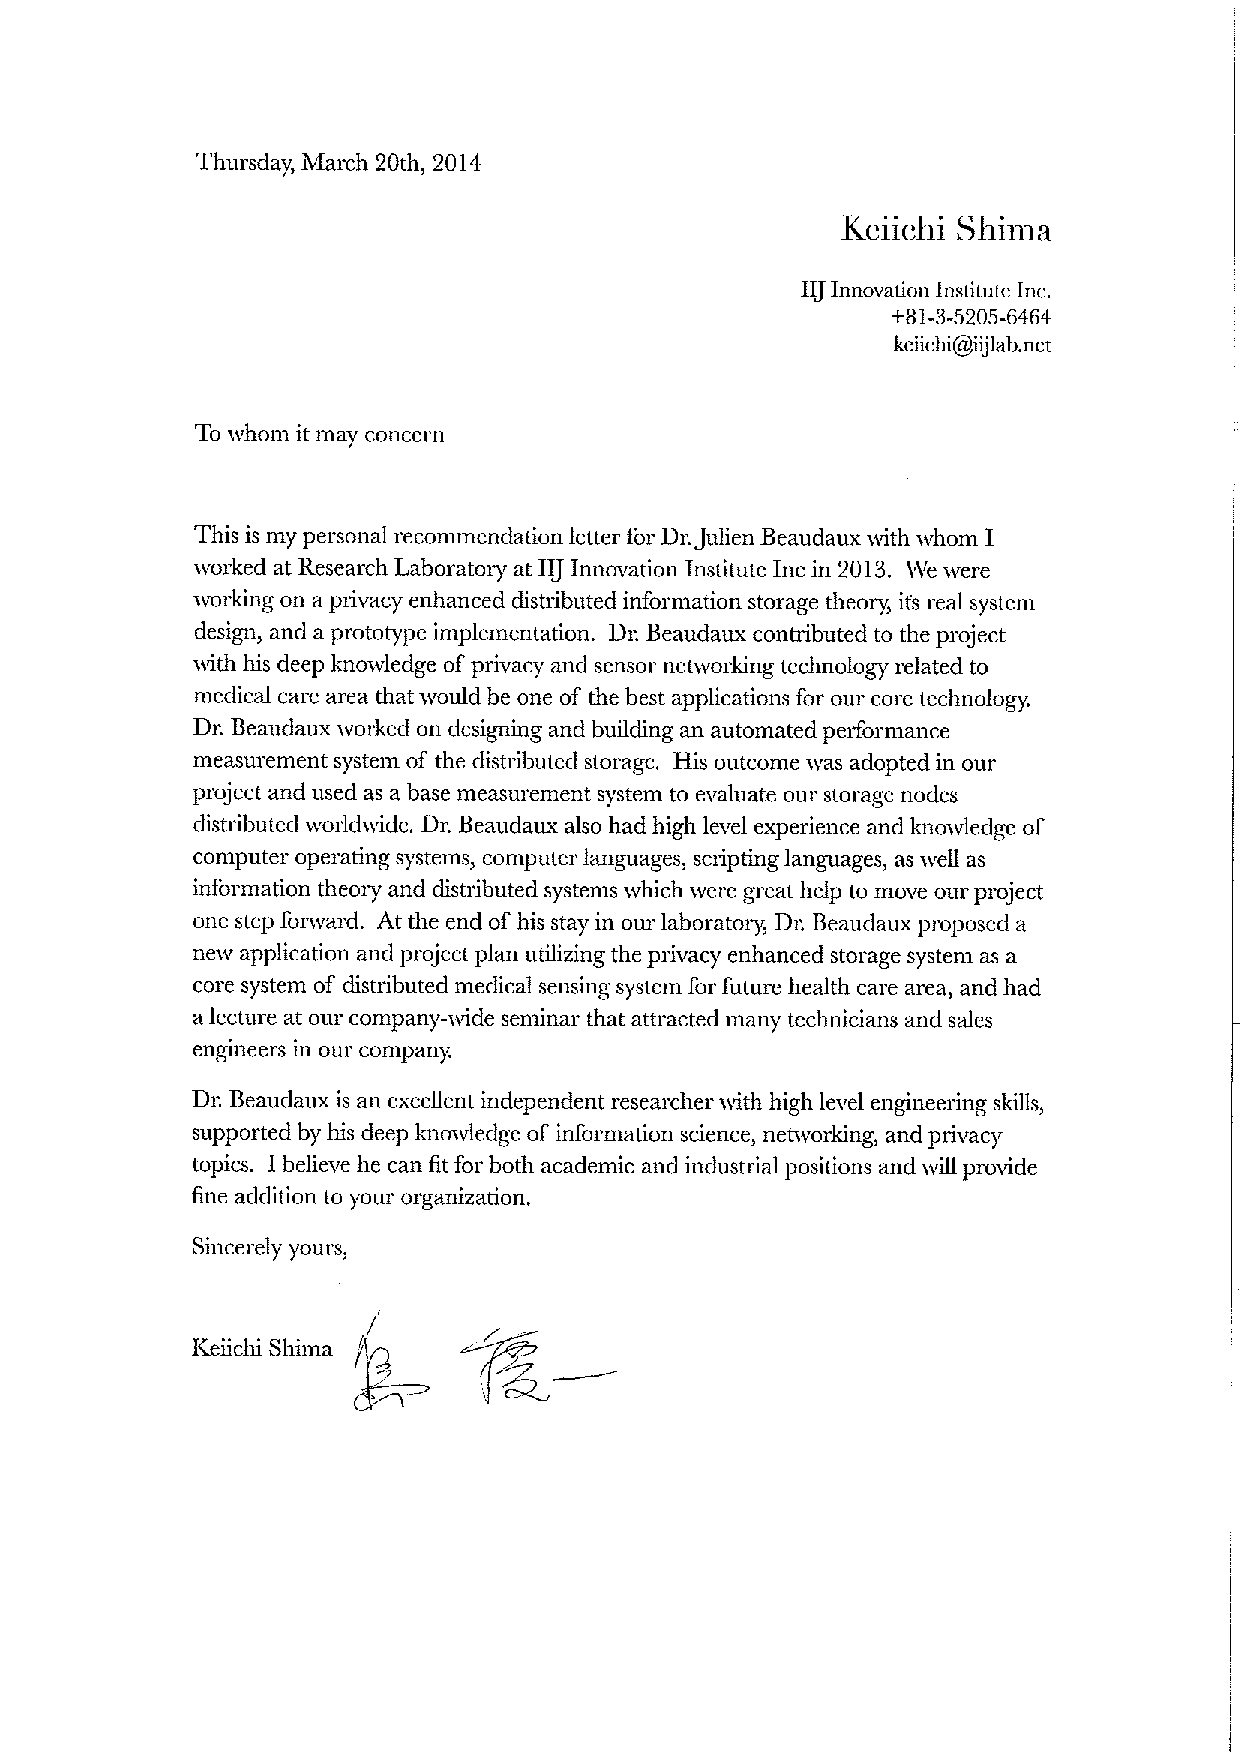
\includepdf[pages={1}]{reco/Reco-IIJ-Shima.pdf}
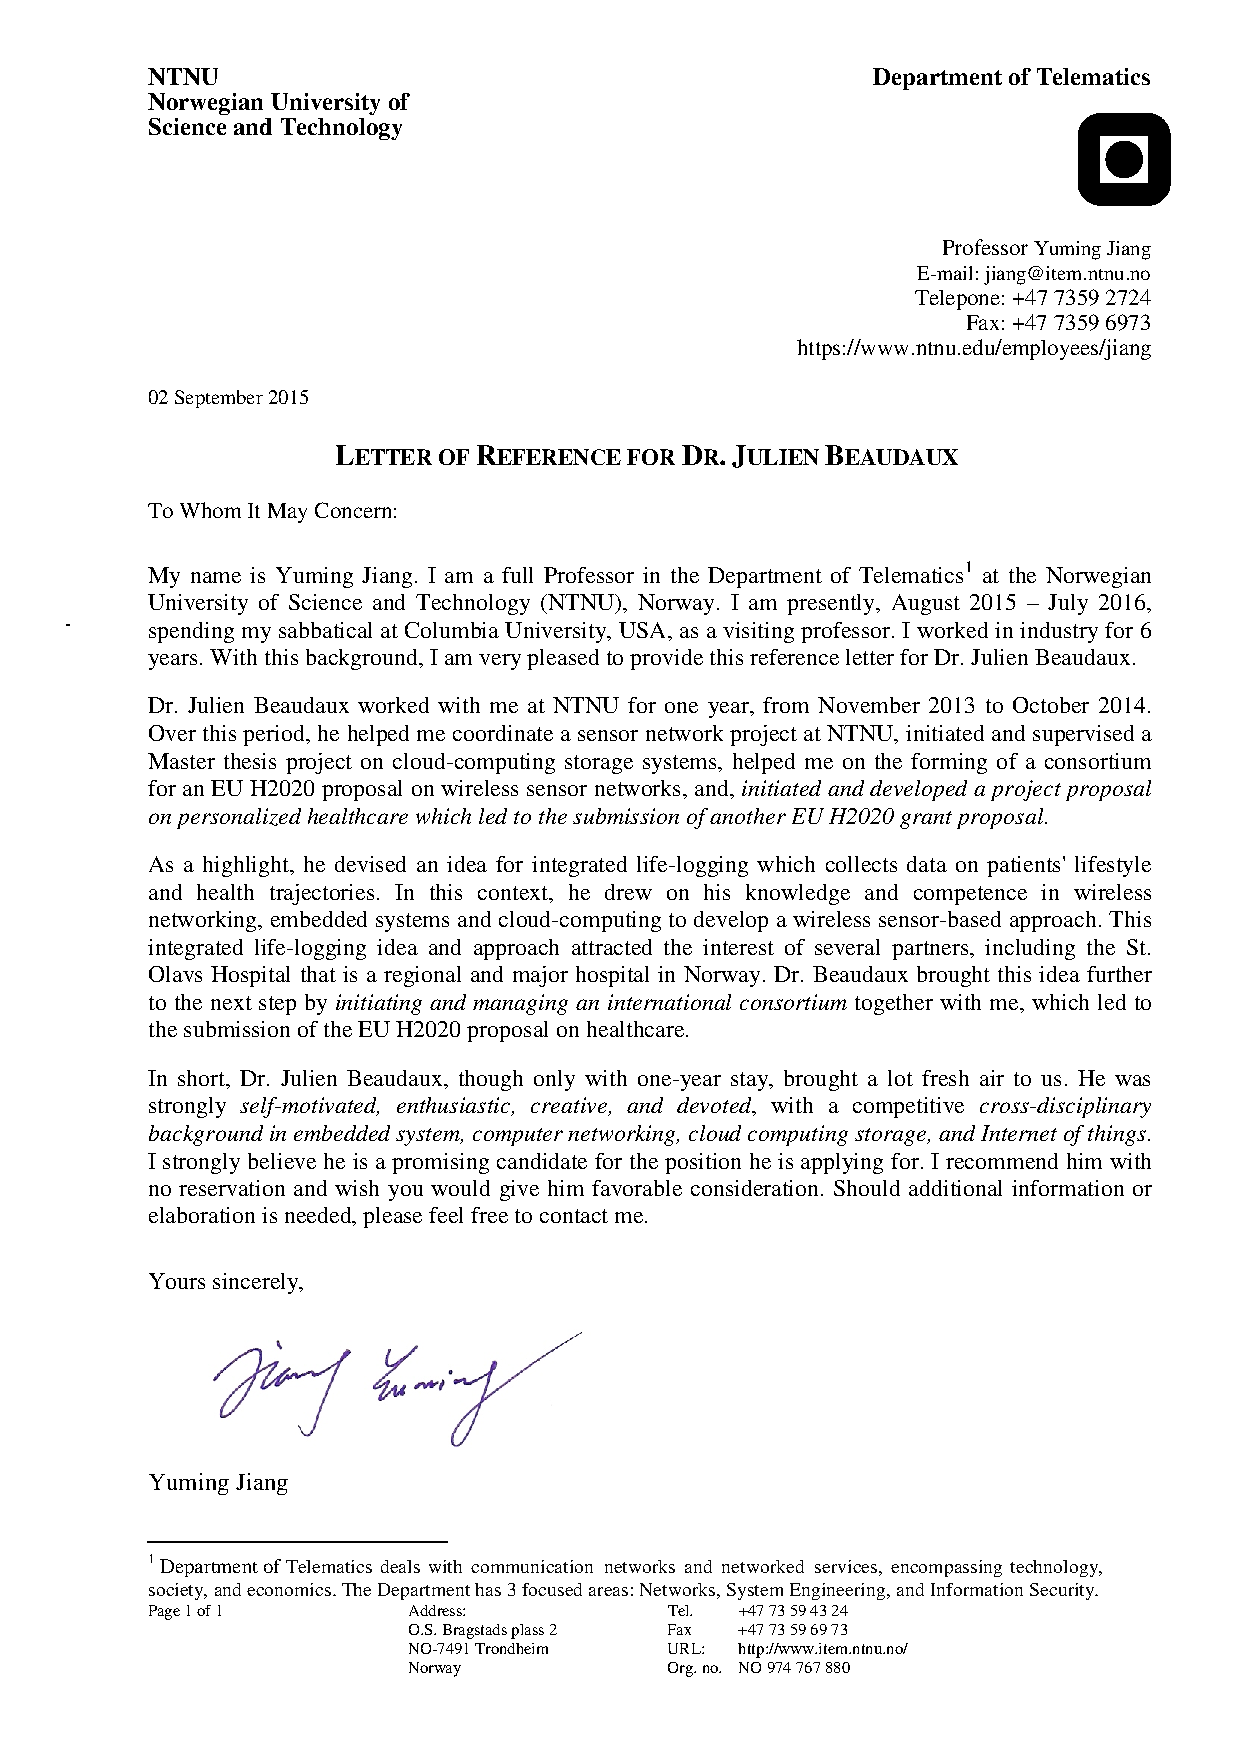
\includepdf[pages={1}]{reco/Reco-NTNU-Jiang.pdf}
\fi

%\end{minipage}
\end{document}